\documentclass[11pt,letterpaper]{article}
\usepackage[lmargin=1in,rmargin=1in,tmargin=1in,bmargin=1in]{geometry}
\usepackage{../style/homework}
\usepackage{../style/commands}
\setbool{quotetype}{true} % True: Side; False: Under
\setbool{hideans}{false} % Student: True; Instructor: False

% -------------------
% Content
% -------------------
\begin{document}

\homework{7: Due 10/17}{The irreducible price of learning is realizing that you do not know.}{James Baldwin}

% Problem 1
\problem{10} Do you think a person's height is a function of time? Do you think a person's salary is a function of their body temperature? For each, explain why or why not. \pspace

\sol Though we may not know what the function is, we know that a person's height is a function of time. Given any time $t$, a person has one possible height---namely, their height at that exact moment. So given an input, there is only one output. \pspace

However, a person's salary is \textit{not} a function of their body temperate. For the majority of your life, your temperature is approximately 98.6$^\circ$F. However, your salary will change over time. So one year you may make \$87,000 and have a normal body temperature of 98.6$^\circ$F, while the next year you get a raise and make \$92,000---while still having (at least some day) a normal body temperature of 98.6$^\circ$F. Therefore, given the body temperature 98.6$^\circ$F, there is more than one possible output salary. Therefore, a person's salary is not a function of their body temperature. 



\newpage



% Problem 2
\problem{10} Determine if the relations $f(x)$ and $g(x)$ shown below are functions. Explain why or why not. If the relation is a function, compute the functions value at $x= -4.1$. 
	\[
	\begin{aligned}
	f(x)&= 198.3 - 17.3x \\[0.3cm]
	g(x)&= 4x^2 + 16.1x - 10.3
	\end{aligned}
	\] \pspace

\sol We know that both $f(x)$ and $g(x)$ are functions: given an input, $x$, there is only one output---namely, the one obtained by `plugging in' $x$ and following order of operations. We have\dots
	\[
	\begin{aligned}
	f(-4.1)&= 198.3 - 17.3(-4.1)= 198.3 - (-70.93)= 198.3 + 70.93= 269.23 \\[0.3cm]
	g(-4.1)&= 4(-4.1)^2 + 16.1(-4.1) - 10.3= 4(16.81) - 66.01 - 10.3= 67.24 - 66.01 - 10.3= -9.07
	\end{aligned}
	\]



\newpage



 % Problem 3
\problem{10} Plot the function $f(x):= \frac{1}{2}x - 5$, being as accurate as possible. 
	\[
	\fbox{
	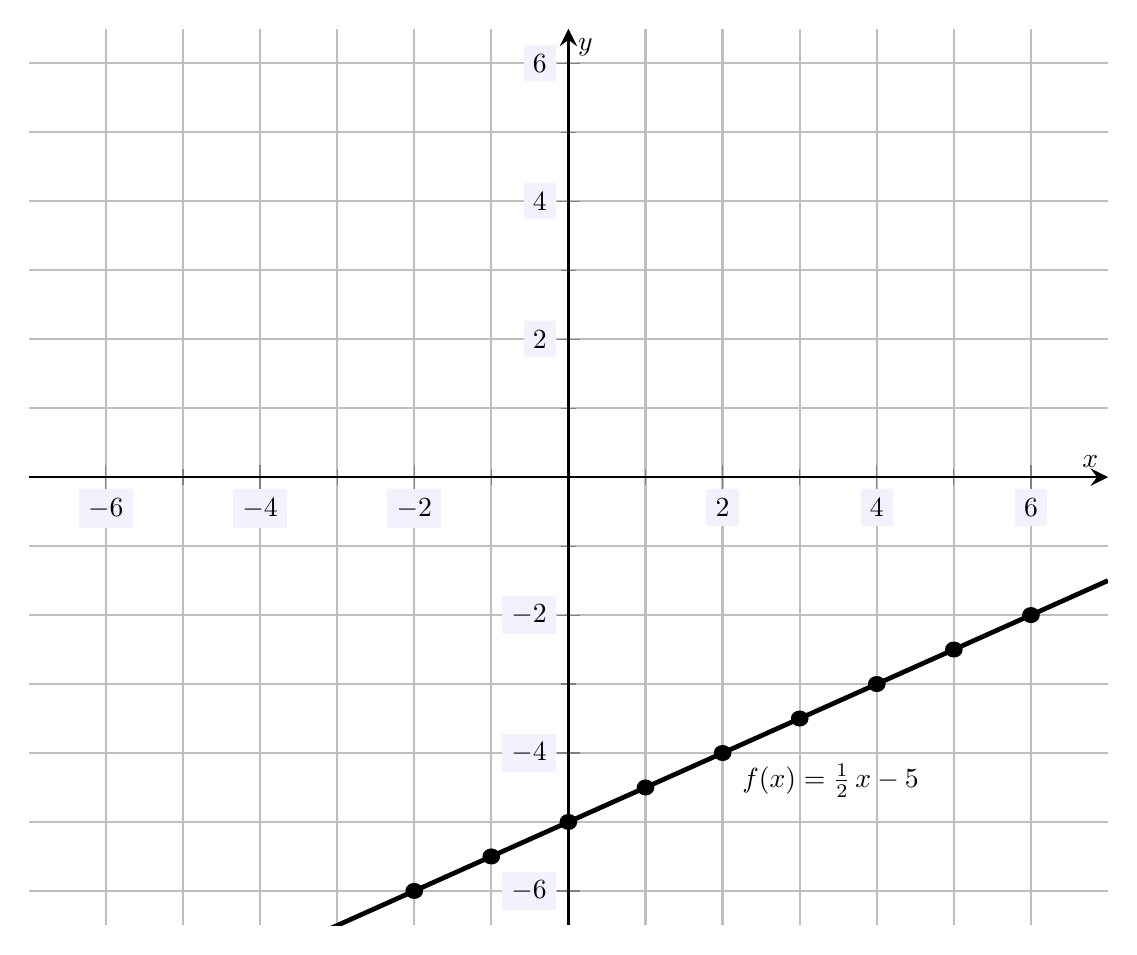
\begin{tikzpicture}[scale=2,every node/.style={scale=0.5}]
	\begin{axis}[
	grid=both,
	axis lines=middle,
	ticklabel style={fill=blue!5!white},
	xmin= -7, xmax=7,
	ymin= -6.5, ymax=6.5,
	xtick={-6,-4,-2,0,2,4,6},
	ytick={-6,-4,-2,0,2,4,6},
	minor tick = {-5,-3,...,5},
	xlabel=\(x\),ylabel=\(y\),
	]
	\addplot[domain=-7:7, samples=100,line width=0.03cm] (x,1/2*x - 5);
	\draw[fill=black] (-2,-12/2) circle (0.1);
	\draw[fill=black] (-1,-11/2) circle (0.1);
	\draw[fill=black] (0,-10/2) circle (0.1);
	\draw[fill=black] (1,-9/2) circle (0.1);
	\draw[fill=black] (2,-8/2) circle (0.1);
	\draw[fill=black] (3,-7/2) circle (0.1);
	\draw[fill=black] (4,-6/2) circle (0.1);
	\draw[fill=black] (5,-5/2) circle (0.1);
	\draw[fill=black] (6,-4/2) circle (0.1);
	\node at (3.4, -4.4) {$f(x)= \frac{1}{2}\,x - 5$};
	\end{axis}
	\end{tikzpicture}
	}
	\]

\sol We have\dots \par
	\begin{table}[!ht]
	\centering
	\begin{tabular}{r||rrrrrrrrrrrrrrr}
	$x$ & $-7$ & $-6$ & $-5$ & $-4$ & $-3$ & $-2$ & $-1$ & $0$ & $1$ & $2$ & $3$ & $4$& $5$ & $6$ & $7$ \\ \hline
	$f(x)$& $-\frac{17}{2}$ & $-8$ & $-\frac{15}{2}$ & $-7$ & $-\frac{13}{2}$ & $-6$ & $-\frac{11}{2}$ & $-5$ & $-\frac{9}{2}$ & $-4$ & $-\frac{7}{2}$ & $-3$ & $-\frac{5}{2}$ & $-2$ & $-\frac{3}{2}$
	\end{tabular}
	\end{table}



\newpage



% Problem 4
\problem{10} Plot the function $f(x):= -x^2 + 4x - 1$, being as accurate as possible. 
	\[
	\fbox{
	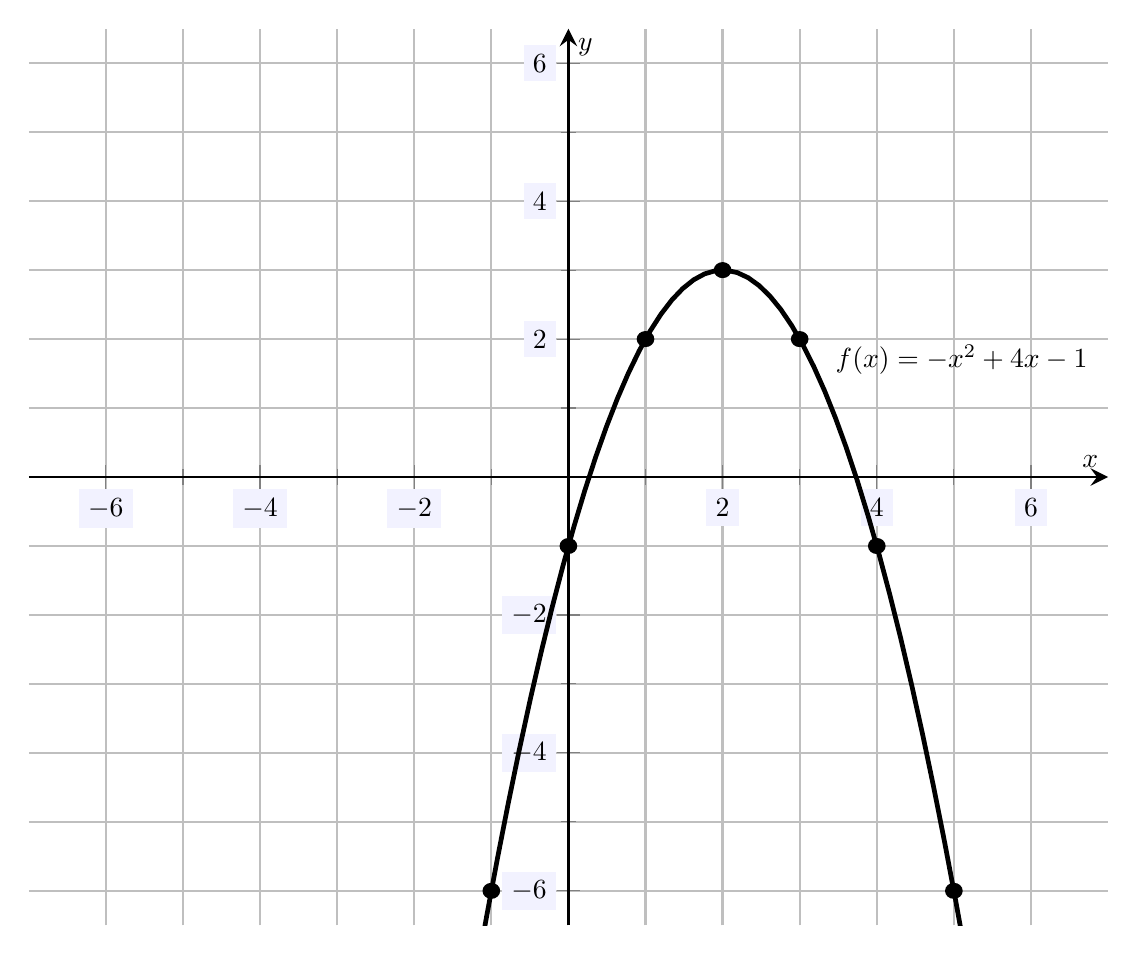
\begin{tikzpicture}[scale=2,every node/.style={scale=0.5}]
	\begin{axis}[
	grid=both,
	axis lines=middle,
	ticklabel style={fill=blue!5!white},
	xmin= -7, xmax=7,
	ymin= -6.5, ymax=6.5,
	xtick={-6,-4,-2,0,2,4,6},
	ytick={-6,-4,-2,0,2,4,6},
	minor tick = {-5,-3,...,5},
	xlabel=\(x\),ylabel=\(y\),
	]
	\addplot[domain=-7:7, samples=100,line width=0.03cm] (x,-x^2 + 4*x - 1);
	\draw[fill=black] (-1,-6) circle (0.1);
	\draw[fill=black] (0,-1) circle (0.1);
	\draw[fill=black] (1,2) circle (0.1);
	\draw[fill=black] (2,3) circle (0.1);
	\draw[fill=black] (3,2) circle (0.1);
	\draw[fill=black] (4,-1) circle (0.1);
	\draw[fill=black] (5,-6) circle (0.1);
	\node at (5.1,1.7) {$f(x)= -x^2 + 4x - 1$};
	\end{axis}
	\end{tikzpicture}
	}
	\]

\sol We have\dots \par
	\begin{table}[!ht]
	\centering
	\begin{tabular}{r||rrrrrrrrrrrrrrr}
	$x$ & $-7$ & $-6$ & $-5$ & $-4$ & $-3$ & $-2$ & $-1$ & $0$ & $1$ & $2$ & $3$ & $4$& $5$ & $6$ & $7$ \\ \hline
	$f(x)$& $-78$ & $-61$ & $-46$ & $-33$ & $-22$ & $-13$ & $-6$ & $-1$ & $2$ & $3$ & $2$ & $-1$ & $-6$ & $-13$ & $-22$
	\end{tabular}
	\end{table}



\end{document}